% Options for packages loaded elsewhere
\PassOptionsToPackage{unicode}{hyperref}
\PassOptionsToPackage{hyphens}{url}
%
\documentclass[
]{article}
\usepackage{lmodern}
\usepackage{amssymb,amsmath}
\usepackage{ifxetex,ifluatex}
\ifnum 0\ifxetex 1\fi\ifluatex 1\fi=0 % if pdftex
  \usepackage[T1]{fontenc}
  \usepackage[utf8]{inputenc}
  \usepackage{textcomp} % provide euro and other symbols
\else % if luatex or xetex
  \usepackage{unicode-math}
  \defaultfontfeatures{Scale=MatchLowercase}
  \defaultfontfeatures[\rmfamily]{Ligatures=TeX,Scale=1}
\fi
% Use upquote if available, for straight quotes in verbatim environments
\IfFileExists{upquote.sty}{\usepackage{upquote}}{}
\IfFileExists{microtype.sty}{% use microtype if available
  \usepackage[]{microtype}
  \UseMicrotypeSet[protrusion]{basicmath} % disable protrusion for tt fonts
}{}
\makeatletter
\@ifundefined{KOMAClassName}{% if non-KOMA class
  \IfFileExists{parskip.sty}{%
    \usepackage{parskip}
  }{% else
    \setlength{\parindent}{0pt}
    \setlength{\parskip}{6pt plus 2pt minus 1pt}}
}{% if KOMA class
  \KOMAoptions{parskip=half}}
\makeatother
\usepackage{xcolor}
\IfFileExists{xurl.sty}{\usepackage{xurl}}{} % add URL line breaks if available
\IfFileExists{bookmark.sty}{\usepackage{bookmark}}{\usepackage{hyperref}}
\hypersetup{
  pdftitle={Running CatalogueExport on Your CDM},
  pdfauthor={Peter Rijnbeek},
  hidelinks,
  pdfcreator={LaTeX via pandoc}}
\urlstyle{same} % disable monospaced font for URLs
\usepackage[margin=1in]{geometry}
\usepackage{color}
\usepackage{fancyvrb}
\newcommand{\VerbBar}{|}
\newcommand{\VERB}{\Verb[commandchars=\\\{\}]}
\DefineVerbatimEnvironment{Highlighting}{Verbatim}{commandchars=\\\{\}}
% Add ',fontsize=\small' for more characters per line
\usepackage{framed}
\definecolor{shadecolor}{RGB}{248,248,248}
\newenvironment{Shaded}{\begin{snugshade}}{\end{snugshade}}
\newcommand{\AlertTok}[1]{\textcolor[rgb]{0.94,0.16,0.16}{#1}}
\newcommand{\AnnotationTok}[1]{\textcolor[rgb]{0.56,0.35,0.01}{\textbf{\textit{#1}}}}
\newcommand{\AttributeTok}[1]{\textcolor[rgb]{0.77,0.63,0.00}{#1}}
\newcommand{\BaseNTok}[1]{\textcolor[rgb]{0.00,0.00,0.81}{#1}}
\newcommand{\BuiltInTok}[1]{#1}
\newcommand{\CharTok}[1]{\textcolor[rgb]{0.31,0.60,0.02}{#1}}
\newcommand{\CommentTok}[1]{\textcolor[rgb]{0.56,0.35,0.01}{\textit{#1}}}
\newcommand{\CommentVarTok}[1]{\textcolor[rgb]{0.56,0.35,0.01}{\textbf{\textit{#1}}}}
\newcommand{\ConstantTok}[1]{\textcolor[rgb]{0.00,0.00,0.00}{#1}}
\newcommand{\ControlFlowTok}[1]{\textcolor[rgb]{0.13,0.29,0.53}{\textbf{#1}}}
\newcommand{\DataTypeTok}[1]{\textcolor[rgb]{0.13,0.29,0.53}{#1}}
\newcommand{\DecValTok}[1]{\textcolor[rgb]{0.00,0.00,0.81}{#1}}
\newcommand{\DocumentationTok}[1]{\textcolor[rgb]{0.56,0.35,0.01}{\textbf{\textit{#1}}}}
\newcommand{\ErrorTok}[1]{\textcolor[rgb]{0.64,0.00,0.00}{\textbf{#1}}}
\newcommand{\ExtensionTok}[1]{#1}
\newcommand{\FloatTok}[1]{\textcolor[rgb]{0.00,0.00,0.81}{#1}}
\newcommand{\FunctionTok}[1]{\textcolor[rgb]{0.00,0.00,0.00}{#1}}
\newcommand{\ImportTok}[1]{#1}
\newcommand{\InformationTok}[1]{\textcolor[rgb]{0.56,0.35,0.01}{\textbf{\textit{#1}}}}
\newcommand{\KeywordTok}[1]{\textcolor[rgb]{0.13,0.29,0.53}{\textbf{#1}}}
\newcommand{\NormalTok}[1]{#1}
\newcommand{\OperatorTok}[1]{\textcolor[rgb]{0.81,0.36,0.00}{\textbf{#1}}}
\newcommand{\OtherTok}[1]{\textcolor[rgb]{0.56,0.35,0.01}{#1}}
\newcommand{\PreprocessorTok}[1]{\textcolor[rgb]{0.56,0.35,0.01}{\textit{#1}}}
\newcommand{\RegionMarkerTok}[1]{#1}
\newcommand{\SpecialCharTok}[1]{\textcolor[rgb]{0.00,0.00,0.00}{#1}}
\newcommand{\SpecialStringTok}[1]{\textcolor[rgb]{0.31,0.60,0.02}{#1}}
\newcommand{\StringTok}[1]{\textcolor[rgb]{0.31,0.60,0.02}{#1}}
\newcommand{\VariableTok}[1]{\textcolor[rgb]{0.00,0.00,0.00}{#1}}
\newcommand{\VerbatimStringTok}[1]{\textcolor[rgb]{0.31,0.60,0.02}{#1}}
\newcommand{\WarningTok}[1]{\textcolor[rgb]{0.56,0.35,0.01}{\textbf{\textit{#1}}}}
\usepackage{graphicx,grffile}
\makeatletter
\def\maxwidth{\ifdim\Gin@nat@width>\linewidth\linewidth\else\Gin@nat@width\fi}
\def\maxheight{\ifdim\Gin@nat@height>\textheight\textheight\else\Gin@nat@height\fi}
\makeatother
% Scale images if necessary, so that they will not overflow the page
% margins by default, and it is still possible to overwrite the defaults
% using explicit options in \includegraphics[width, height, ...]{}
\setkeys{Gin}{width=\maxwidth,height=\maxheight,keepaspectratio}
% Set default figure placement to htbp
\makeatletter
\def\fps@figure{htbp}
\makeatother
\setlength{\emergencystretch}{3em} % prevent overfull lines
\providecommand{\tightlist}{%
  \setlength{\itemsep}{0pt}\setlength{\parskip}{0pt}}
\setcounter{secnumdepth}{5}

\title{Running CatalogueExport on Your CDM}
\author{Peter Rijnbeek}
\date{2020-12-12}

\begin{document}
\maketitle

{
\setcounter{tocdepth}{3}
\tableofcontents
}
\hypertarget{introduction}{%
\section{Introduction}\label{introduction}}

In this vignette we cover how to run the CatlogueExport package on your
Common Data Model (CDM) database in order to characterize the dataset
and create a result file that can be uploaded in the
\href{https://portal.ehden.eu}{EHDEN Catalogue}. It is a requirement for
all EHDEN sites to run CatalogueExport on their CDM datasets to ensure
researchers can evaluate study feasibility and contextualize study
results.

\hypertarget{general-approach}{%
\section{General Approach}\label{general-approach}}

The CatalogueExport package consists of:

\begin{enumerate}
\def\labelenumi{\arabic{enumi}.}
\tightlist
\item
  The \textbf{catalogueExport} function runs a set of SQL scripts to
  characterize the domains and concepts of the CDM.
\item
  The \textbf{createIndices} function creates table indices for the
  achilles tables, which can help improve query performance.
\item
  The \textbf{validateSchema} function compares your CDM schema against
  the OMOP CDM specification.
\item
  The \textbf{getAnalysisDetails} function provides descriptions about
  the full set of Achilles analyses.
\item
  The \textbf{dropAllScratchTables} function is useful only for
  multi-threaded mode. It can clear any leftover staging tables.
\end{enumerate}

\hypertarget{sql-only-mode}{%
\subsection{SQL Only Mode}\label{sql-only-mode}}

In most functions, you can specify \texttt{sqlOnly\ =\ TRUE} in order to
produce the SQL without executing it, which can be useful if you'd like
to examine the SQL closely or debug something. The SQL files are stored
in the \texttt{outputFolder}.

\hypertarget{logging}{%
\subsection{Logging}\label{logging}}

File and console logging is enabled across most functions. The status of
each step is logged into files in the \texttt{outputFolder}. You can
review the files in a common text editor, or use the Shiny Application
from the \texttt{ParallelLogger} package to view them more
interactively.

\begin{Shaded}
\begin{Highlighting}[]
\NormalTok{ParallelLogger}\OperatorTok{::}\KeywordTok{launchLogViewer}\NormalTok{(}\DataTypeTok{logFileName =} \StringTok{"output/log_catalogueExport.txt"}\NormalTok{)}
\end{Highlighting}
\end{Shaded}

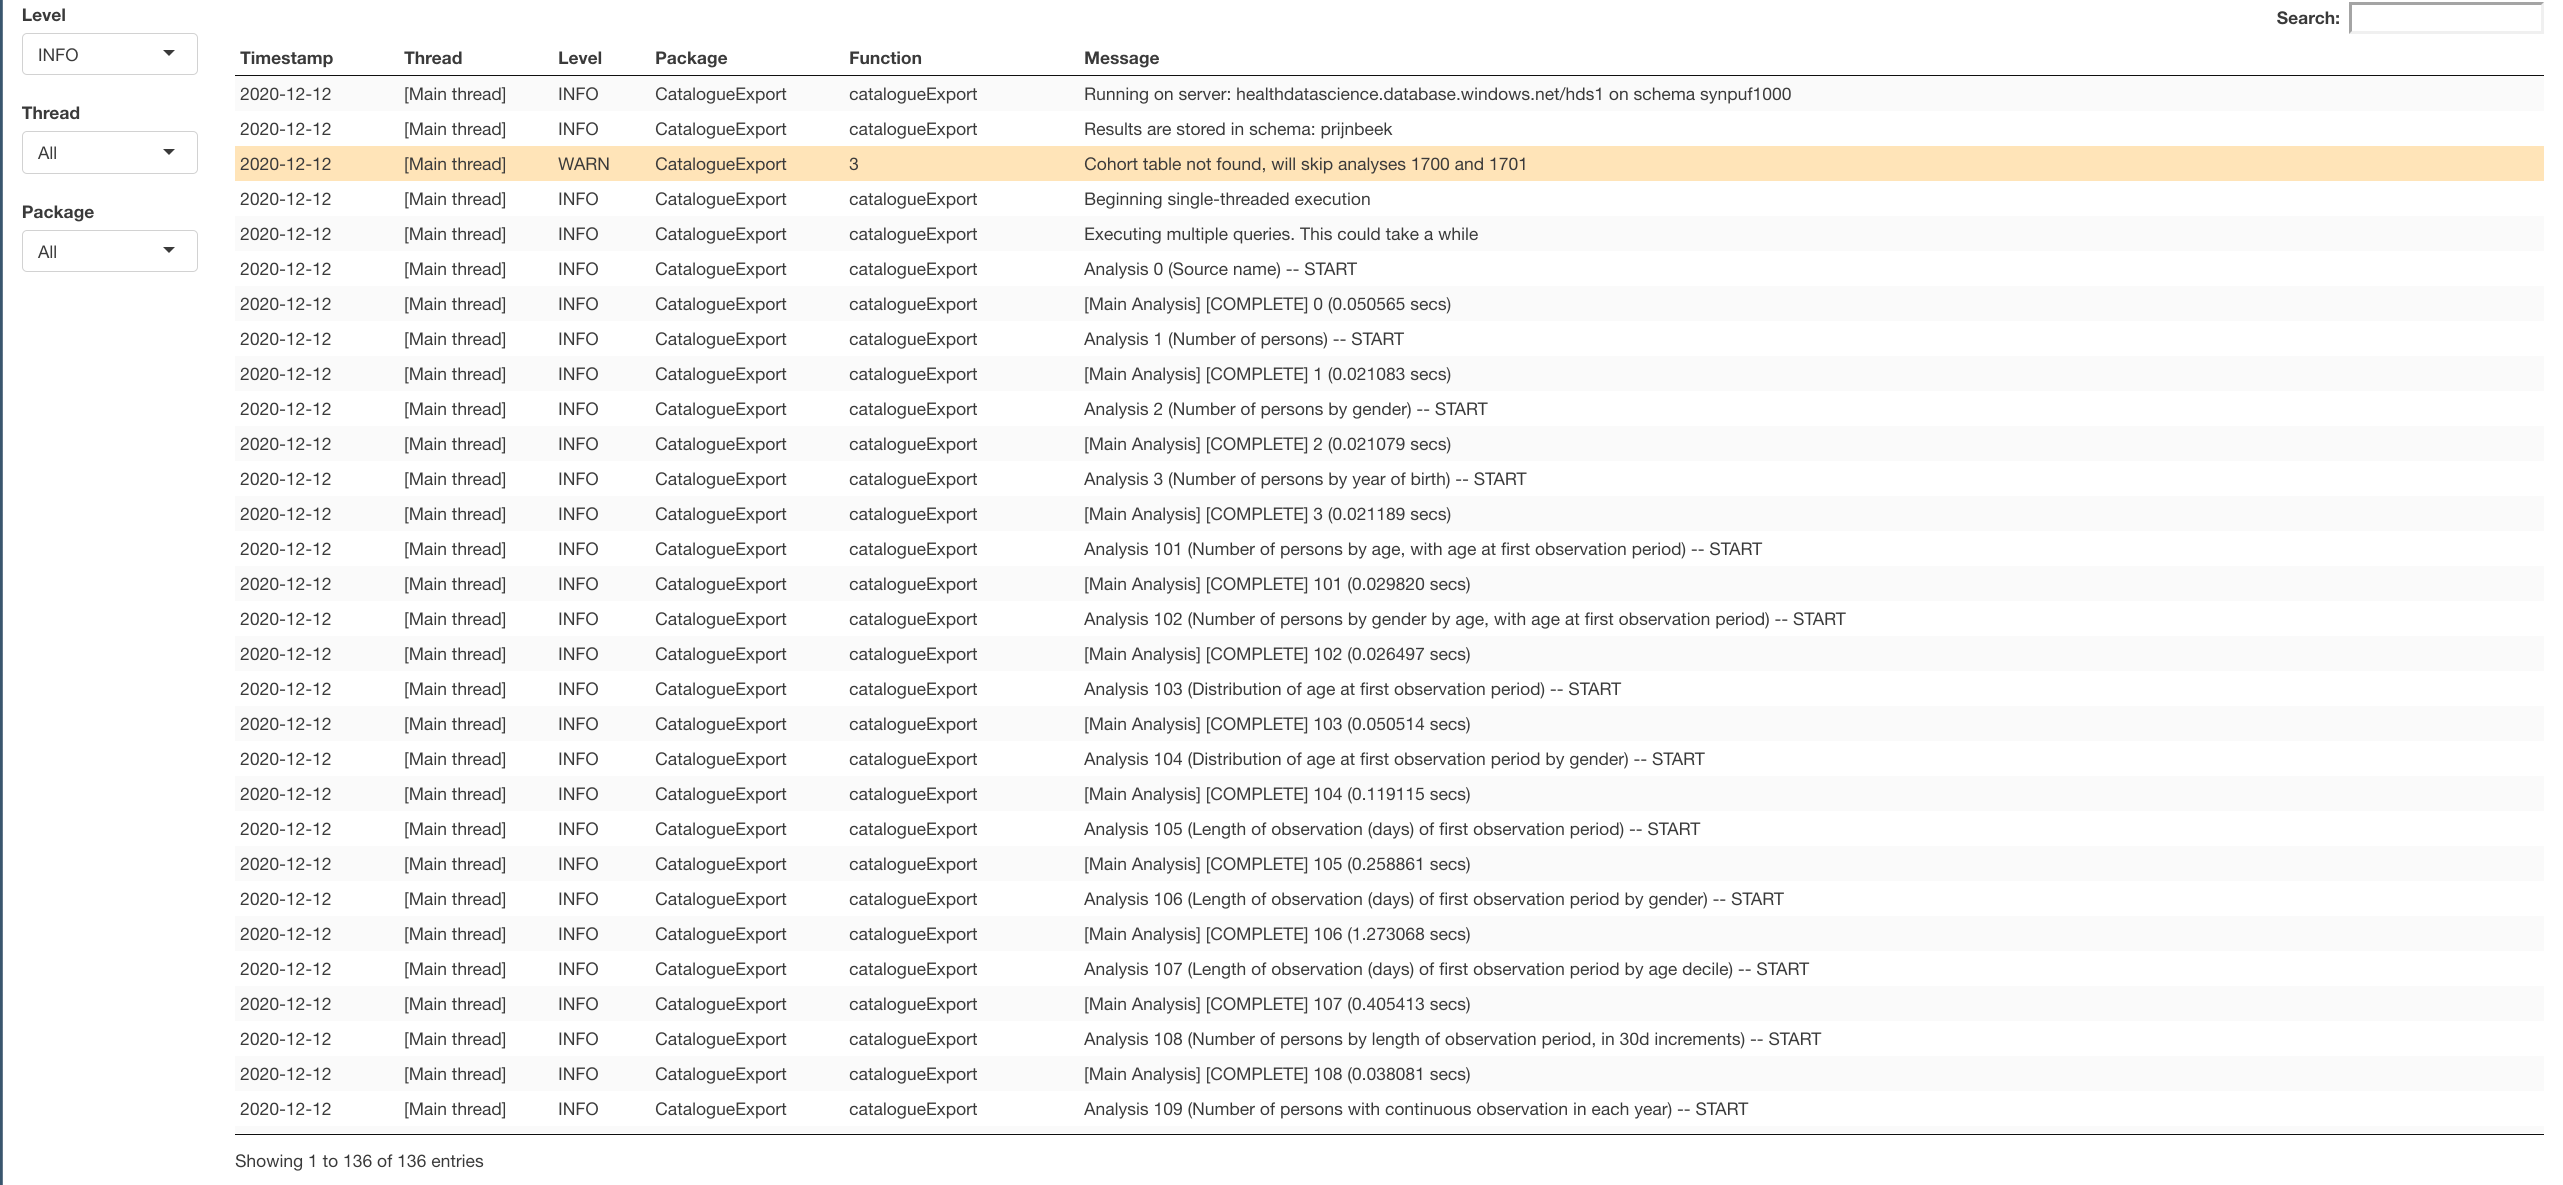
\includegraphics{../inst/doc/logging_screenshot.png}

\hypertarget{verbose-mode}{%
\subsection{Verbose Mode}\label{verbose-mode}}

The \texttt{verboseMode} parameter can be set to FALSE if you'd like
less details about the function execution to appear in the console.
Either way, all details are written to the log files. By default, this
is set to TRUE.

\hypertarget{preparation-for-running-catalogueexport}{%
\subsection{Preparation for running
CatalogueExport}\label{preparation-for-running-catalogueexport}}

In order to run the package, you will need to determine if you'd like
the tables and staging tables to be stored in schemas that are separate
from your CDM's schema (recommended), or within the same schema as the
CDM.

\hypertarget{multi-threaded-vs-single-threaded}{%
\subsubsection{Multi-Threaded vs
Single-Threaded}\label{multi-threaded-vs-single-threaded}}

As most of the queries can run independently, we have added a
multi-threaded mode to allow for more than 1 SQL script to execute at a
time. This is particularly useful for massively parallel processing
(MPP) platforms such as Amazon Redshift and Microsoft PDW. It may not be
beneficial for traditional SQL platforms, so only use the multi-threaded
mode if confident it can be useful.

Further, while multiple threads can help performance in MPP platforms,
there can be diminishing returns as the cluster has a finite number of
concurrency slots to handle the queries. A rule of thumb: most likely
you should not use more than 10.

In the multi-threaded mode, all scripts produce permanent staging
tables, whereas in the single-threaded mode, the scripts produce
temporary staging tables. In both, the staging tables are merged to
produce the final Achilles tables.

\hypertarget{validate-your-cdm-schema}{%
\subsubsection{Validate your CDM
schema}\label{validate-your-cdm-schema}}

Before you run \textbf{catalogueExport}, it may be useful to verify that
your CDM schema conforms to the OMOP CDM specification. This can quickly
identify issues with your CDM ahead of time. Refer to the
\href{https://github.com/OHDSI/CommonDataModel}{Common Data Model repo}
to identify which version of the CDM you intend to validate against.

\begin{Shaded}
\begin{Highlighting}[]
\NormalTok{connectionDetails <-}\StringTok{ }\KeywordTok{createConnectionDetails}\NormalTok{(}\DataTypeTok{dbms =} \StringTok{"postgresql"}\NormalTok{, }
                                             \DataTypeTok{server =} \StringTok{"localhost/synpuf"}\NormalTok{, }
                                             \DataTypeTok{user =} \StringTok{"cdm_user"}\NormalTok{, }
                                             \DataTypeTok{password =} \StringTok{"cdm_password"}\NormalTok{)}
\KeywordTok{validateSchema}\NormalTok{(}\DataTypeTok{connectionDetails =}\NormalTok{ connectionDetails, }
               \DataTypeTok{cdmDatabaseSchema =} \StringTok{"cdm"}\NormalTok{, }
               \DataTypeTok{resultsDatabaseSchema =} \StringTok{"results"}\NormalTok{, }
               \DataTypeTok{cdmVersion =} \FloatTok{5.3}\NormalTok{, }
               \DataTypeTok{runCostAnalysis =} \OtherTok{TRUE}\NormalTok{, }
               \DataTypeTok{outputFolder =} \StringTok{"output"}\NormalTok{, }
               \DataTypeTok{sqlOnly =} \OtherTok{FALSE}\NormalTok{)}
\end{Highlighting}
\end{Shaded}

\hypertarget{parameters-both-modes}{%
\section{Parameters (Both Modes)}\label{parameters-both-modes}}

The following sub-sections describe the optional parameters in
\textbf{catalogueExport} that can be configured, regardless of whether
you run the function in single- or multi-threaded mode.

\hypertarget{staging-table-prefix}{%
\subsection{Staging Table Prefix}\label{staging-table-prefix}}

To keep the staging tables organized, the \textbf{catalogueExport}
function will use a table prefix of ``tmpach'' by default, but you can
choose a different one using the \texttt{tempAchillesPrefix} parameter.
This is useful for database platforms like Oracle, which limit the
length of table names.

\hypertarget{source-name}{%
\subsection{Source Name}\label{source-name}}

The \texttt{sourceName} parameter is used to assign the name of the
dataset to the CatalogueExport results. It is used in the Dashboard
pages in the visualisations in the database catalogue. If you set this
to \texttt{NULL}, the \textbf{catalogueExport} function will try to
obtain the source name from the CDM\_SOURCE table.

\hypertarget{create-table}{%
\subsection{Create Table}\label{create-table}}

The \texttt{createTable} parameter, when set to \texttt{TRUE}, drops any
existing results tables and builds new ones. If set to \texttt{FALSE},
these tables will persist, and the \textbf{catalogueExport} function
will just insert new data to them.

\hypertarget{limiting-the-analyses}{%
\subsection{Limiting the Analyses}\label{limiting-the-analyses}}

By default, the \textbf{catalogueExport} function runs all analyses
detailed in the \texttt{getAnalysisDetails} function. However, it may be
useful to focus on a subset of analyses rather than running the whole
set. This can be accomplished by specifying analysis Ids in the
\texttt{analysisIds} parameter.

\hypertarget{small-cell-count}{%
\subsection{Small Cell Count}\label{small-cell-count}}

To avoid patient identifiability, you can establish the minimum cell
size that should be kept in the result tables. Cells with small counts
(less than or equal to the value of the \texttt{smallCellCount}
parameter) are deleted. By default, this is set to 5. However, set to
NULL if you don't want any deletions. Note that all counts on
concept\_id level are rounded up to the nearest multiple of 100
independent on this setting.

\hypertarget{drop-scratch-tables}{%
\subsection{Drop Scratch Tables}\label{drop-scratch-tables}}

\emph{See the Post-Processing section to read about how to run this step
separately}

\emph{This parameter is only necessary if running in multi-threaded
mode}

The \texttt{dropScratchTables} parameter, if set to \texttt{TRUE}, will
drop all staging tables created during the execution of
\textbf{catalogueExport} in multi-threaded mode.

\hypertarget{create-indices}{%
\subsection{Create Indices}\label{create-indices}}

\emph{See the Post-Processing section to read about how to run this step
separately}

The \texttt{createIndices} parameter, if set to \texttt{TRUE}, will
result in indices on the results tables to be created in order to
improve query performance.

\hypertarget{return-value}{%
\subsection{Return Value}\label{return-value}}

When running \textbf{catalogueExport}, the return value, if you assign a
variable to the function call, is a list object in which metadata about
the execution and all of the SQL scripts executed are attributes. You
can also run the function call without assigning a variable to it, so
that no values are printed or returned.

\hypertarget{running-in-single-threaded-mode}{%
\section{Running in Single-Threaded
Mode}\label{running-in-single-threaded-mode}}

In single-threaded mode, there is no need to set a
\texttt{scratchDatabaseSchema}, as temporary tables will be used.

\begin{Shaded}
\begin{Highlighting}[]
\NormalTok{connectionDetails <-}\StringTok{ }\KeywordTok{createConnectionDetails}\NormalTok{(}\DataTypeTok{dbms =} \StringTok{"postgresql"}\NormalTok{, }
                                             \DataTypeTok{server =} \StringTok{"localhost/synpuf"}\NormalTok{, }
                                             \DataTypeTok{user =} \StringTok{"cdm_user"}\NormalTok{, }
                                             \DataTypeTok{password =} \StringTok{"cdm_password"}\NormalTok{)}
\KeywordTok{achilles}\NormalTok{(}\DataTypeTok{connectionDetails =}\NormalTok{ connectionDetails, }
         \DataTypeTok{cdmDatabaseSchema =} \StringTok{"cdm"}\NormalTok{, }
         \DataTypeTok{resultsDatabaseSchema =} \StringTok{"results"}\NormalTok{, }
         \DataTypeTok{vocabDatabaseSchema =} \StringTok{"vocab"}\NormalTok{, }
         \DataTypeTok{sourceName =} \StringTok{"Synpuf"}\NormalTok{, }
         \DataTypeTok{cdmVersion =} \FloatTok{5.3}\NormalTok{, }
         \DataTypeTok{numThreads =} \DecValTok{1}\NormalTok{)}
\end{Highlighting}
\end{Shaded}

\hypertarget{running-in-multi-threaded-mode}{%
\section{Running in Multi-Threaded
Mode}\label{running-in-multi-threaded-mode}}

In multi-threaded mode, you need to specify
\texttt{scratchDatabaseSchema} and use \textgreater{} 1 for
\texttt{numThreads}.

\begin{Shaded}
\begin{Highlighting}[]
\NormalTok{connectionDetails <-}\StringTok{ }\KeywordTok{createConnectionDetails}\NormalTok{(}\DataTypeTok{dbms =} \StringTok{"postgresql"}\NormalTok{, }
                                             \DataTypeTok{server =} \StringTok{"localhost/synpuf"}\NormalTok{, }
                                             \DataTypeTok{user =} \StringTok{"cdm_user"}\NormalTok{, }
                                             \DataTypeTok{password =} \StringTok{"cdm_password"}\NormalTok{)}
\KeywordTok{achilles}\NormalTok{(}\DataTypeTok{connectionDetails =}\NormalTok{ connectionDetails, }
         \DataTypeTok{cdmDatabaseSchema =} \StringTok{"cdm"}\NormalTok{, }
         \DataTypeTok{resultsDatabaseSchema =} \StringTok{"results"}\NormalTok{, }
         \DataTypeTok{scratchDatabaseSchema =} \StringTok{"scratch"}\NormalTok{, }
         \DataTypeTok{vocabDatabaseSchema =} \StringTok{"vocab"}\NormalTok{, }
         \DataTypeTok{sourceName =} \StringTok{"Synpuf"}\NormalTok{, }
         \DataTypeTok{cdmVersion =} \FloatTok{5.3}\NormalTok{, }
         \DataTypeTok{numThreads =} \DecValTok{5}\NormalTok{)}
\end{Highlighting}
\end{Shaded}

\hypertarget{post-processing}{%
\section{Post-Processing}\label{post-processing}}

This section describes the usage of standalone functions for
post-processing that can be invoked if you did not use them in the
\textbf{catalogueExport} function call.

\hypertarget{creating-indices}{%
\subsection{Creating Indices}\label{creating-indices}}

\emph{Not supported by Amazon Redshift or IBM Netezza; function will
skip this step if using those platforms}

To improve query performance of the results tables, run the
\textbf{createIndices} function.

\begin{Shaded}
\begin{Highlighting}[]
\NormalTok{connectionDetails <-}\StringTok{ }\KeywordTok{createConnectionDetails}\NormalTok{(}\DataTypeTok{dbms =} \StringTok{"postgresql"}\NormalTok{, }
                                             \DataTypeTok{server =} \StringTok{"localhost/synpuf"}\NormalTok{, }
                                             \DataTypeTok{user =} \StringTok{"cdm_user"}\NormalTok{, }
                                             \DataTypeTok{password =} \StringTok{"cdm_password"}\NormalTok{)}
\KeywordTok{createIndices}\NormalTok{(}\DataTypeTok{connectionDetails =}\NormalTok{ connectionDetails, }
              \DataTypeTok{resultsDatabaseSchema =} \StringTok{"results"}\NormalTok{, }
              \DataTypeTok{outputFolder =} \StringTok{"output"}\NormalTok{)}
\end{Highlighting}
\end{Shaded}

\hypertarget{dropping-all-staging-tables-multi-threaded-only}{%
\subsection{Dropping All Staging Tables (Multi-threaded
only)}\label{dropping-all-staging-tables-multi-threaded-only}}

If the \textbf{catalogueExport} execution has errors, or if you did not
enable this step in the call to these functions, use the
\texttt{dropAllScratchTables} function.

\begin{Shaded}
\begin{Highlighting}[]
\NormalTok{connectionDetails <-}\StringTok{ }\KeywordTok{createConnectionDetails}\NormalTok{(}\DataTypeTok{dbms =} \StringTok{"postgresql"}\NormalTok{, }
                                             \DataTypeTok{server =} \StringTok{"localhost/synpuf"}\NormalTok{, }
                                             \DataTypeTok{user =} \StringTok{"cdm_user"}\NormalTok{, }
                                             \DataTypeTok{password =} \StringTok{"cdm_password"}\NormalTok{)}
\KeywordTok{dropAllScratchTables}\NormalTok{(}\DataTypeTok{connectionDetails =}\NormalTok{ connectionDetails, }
                     \DataTypeTok{scratchDatabaseSchema =} \StringTok{"scratch"}\NormalTok{, }\DataTypeTok{numThreads =} \DecValTok{5}\NormalTok{)}
\end{Highlighting}
\end{Shaded}

\hypertarget{upload-results-in-the-database-catalogue}{%
\section{Upload results in the Database
Catalogue}\label{upload-results-in-the-database-catalogue}}

The output file created in you output folder can be uploaded in the
EHDEN Database Catalogue if you have the upload rights for your
database.

\begin{enumerate}
\def\labelenumi{\arabic{enumi}.}
\tightlist
\item
  Login to the EHDEN Portal (\url{https://portal.ehden.eu})
\item
  Navigate to your database and click on ``Dashboard Data Upload'' tab
  (see figure below). The select the file to upload. You can see the
  upload history on this page as ell
\end{enumerate}

All visualisations in the Database Dashboard and the Network Dashboards
will now automatically reflect the new characteristics of your database.
Please rerun this procedure for every CDM update so the dashboard shows
the latest version of your data.

\hypertarget{acknowledgments}{%
\section{Acknowledgments}\label{acknowledgments}}

Considerable part of this work has been used from the \texttt{Achilles}
package.

\begin{Shaded}
\begin{Highlighting}[]
\KeywordTok{citation}\NormalTok{(}\StringTok{"Achilles"}\NormalTok{)}
\end{Highlighting}
\end{Shaded}

\begin{verbatim}
#> 
#> To cite package 'Achilles' in publications use:
#> 
#>   Patrick Ryan, Martijn Schuemie, Vojtech Huser, Chris Knoll, Ajit Londhe and Taha Abdul-Basser (2019). Achilles: Creates Descriptive Statistics
#>   Summary for an Entire OMOP CDM Instance. R package version 1.6.7.
#> 
#> A BibTeX entry for LaTeX users is
#> 
#>   @Manual{,
#>     title = {Achilles: Creates Descriptive Statistics Summary for an Entire OMOP CDM Instance},
#>     author = {Patrick Ryan and Martijn Schuemie and Vojtech Huser and Chris Knoll and Ajit Londhe and Taha Abdul-Basser},
#>     year = {2019},
#>     note = {R package version 1.6.7},
#>   }
\end{verbatim}

For citing the CatalogueExport package please use:

\begin{Shaded}
\begin{Highlighting}[]
\KeywordTok{citation}\NormalTok{(}\StringTok{"CatalogueExport"}\NormalTok{)}
\end{Highlighting}
\end{Shaded}

\begin{verbatim}
#> 
#> To cite package 'CatalogueExport' in publications use:
#> 
#>   Peter Rijnbeek, Patrick Ryan, Martijn Schuemie, Vojtech Huser, Chris Knoll, Ajit Londhe and Taha Abdul-Basser (2020). CatalogueExport: Exports
#>   Descriptive Statistics Summary for the EHDEN Database Catalogue. R package version 1.0.
#> 
#> A BibTeX entry for LaTeX users is
#> 
#>   @Manual{,
#>     title = {CatalogueExport: Exports Descriptive Statistics Summary for the EHDEN Database Catalogue},
#>     author = {Peter Rijnbeek and Patrick Ryan and Martijn Schuemie and Vojtech Huser and Chris Knoll and Ajit Londhe and Taha Abdul-Basser},
#>     year = {2020},
#>     note = {R package version 1.0},
#>   }
\end{verbatim}

\end{document}
